\documentclass[11pt]{article}

\usepackage[a4paper,margin=1in]{geometry}
\usepackage{lmodern}
\usepackage[T1]{fontenc}
\usepackage[utf8]{inputenc}
\usepackage{microtype}
\usepackage{graphicx}
\usepackage{booktabs}
\usepackage{caption}
\usepackage{amsmath}
\usepackage{amssymb}
\usepackage{xcolor}
\usepackage[colorlinks=true,allcolors=black,urlcolor=blue!55!black]{hyperref}

\graphicspath{{../figures/}}

\definecolor{ink}{HTML}{1A1A1A}
\definecolor{muted}{HTML}{6A6A6A}
\definecolor{accent}{HTML}{2B6CB0}
\color{ink}
\captionsetup{font=small,labelfont=bf,labelsep=period}
\setlength{\parskip}{0.45em}
\setlength{\parindent}{0pt}
\renewcommand{\arraystretch}{1.15}

\title{\vspace{-1.5em}\textbf{\Large Genes that work together, travel together}\\[0.35em]
  \large Measuring gene-family coupling from genome content ---\\ tested on simulations, then on 43 bacterial genomes}
\author{ZOMBI2 \,\textbullet\, coupling analysis}
\date{\small 2026-07-05}

\begin{document}
\maketitle
\vspace{-1.4em}

\begin{abstract}\noindent
Bacteria constantly gain new genes (often by picking them up from other bacteria) and lose old
ones. We study a model in which genes that \emph{work together} tend to be gained and lost together,
so they end up present in the same genomes. This report asks two simple questions. \textbf{First},
on simulated data where we know the answer: can we measure the \emph{strength} of this ``togetherness''
just from a table of which genes are in which genomes? We can, and accurately. \textbf{Second}, on a
real dataset of \textbf{43 bacterial genomes} with each gene labelled by its function: do genes of the
same function actually appear together more than chance? They do --- strongly, and led by the genes
for cell motility. Together this is a step toward generating realistic simulated genomes that match
real data, using gene \emph{function} to decide which genes should be coupled.
\end{abstract}

\section{What we are trying to do}

Suppose we have a real dataset: a table saying, for a set of bacterial genomes, which gene families
each genome contains (a \emph{families}\,$\times$\,\emph{genomes} table of presence/absence or copy
numbers). We would like to build a \emph{model} that reproduces this kind of data --- so we can
generate synthetic genomes that look real, and understand the forces that shaped them. The catch is
that our model is complex enough that we cannot write down its likelihood (the probability of the
data given the model), so we cannot fit it by standard means. Instead we use \textbf{Approximate
Bayesian Computation (ABC)}: we simulate data under many settings of the model, and keep the settings
whose simulated data most resemble the real data. No likelihood required.

\section{The model, in words}

Genes come and go along the tree of bacterial species:
\begin{itemize}\setlength\itemsep{0.15em}
\item \textbf{Gain.} A genome can acquire a gene by \emph{horizontal transfer} --- a copy jumps in
from another lineage.
\item \textbf{Loss.} A gene already present can be lost over time.
\item \textbf{Coupling.} Genes that belong to the same functional group help each other. If a gene's
partners are already present, it is (a)~\emph{less likely to be lost}, and (b)~\emph{more likely to
take hold} when it transfers in. The strength of this help is a number we call~$J$: $J=0$ means genes
behave independently, larger~$J$ means tighter coupling.
\end{itemize}
The consequence is that coupled genes tend to be \emph{present together} across genomes. Our goal is
to recover~$J$ from the data. (Everything below uses this full gain-\emph{and}-loss coupling model.)

\section{Can we measure the coupling? (a simulation test)}

Because we cannot test recovery on real data (we don't know the true~$J$ there), we first test it on
simulations, where we set~$J$ ourselves and check whether we get it back.

\textbf{Coupling leaves a visible fingerprint.} When genes are coupled, families in the same group
tend to be present in the same genomes --- so if we compute, for every pair of families, how
correlated their presence is, coupled families light up as blocks (Fig.~\ref{fig:heat}a). Uncoupled
families show no such blocks (Fig.~\ref{fig:heat}b). Reassuringly, the family tree itself does
\emph{not} create these blocks by accident (related genomes share genes, which could mimic coupling):
on this tree, uncoupled families show essentially no correlation.

\begin{figure}[h]\centering
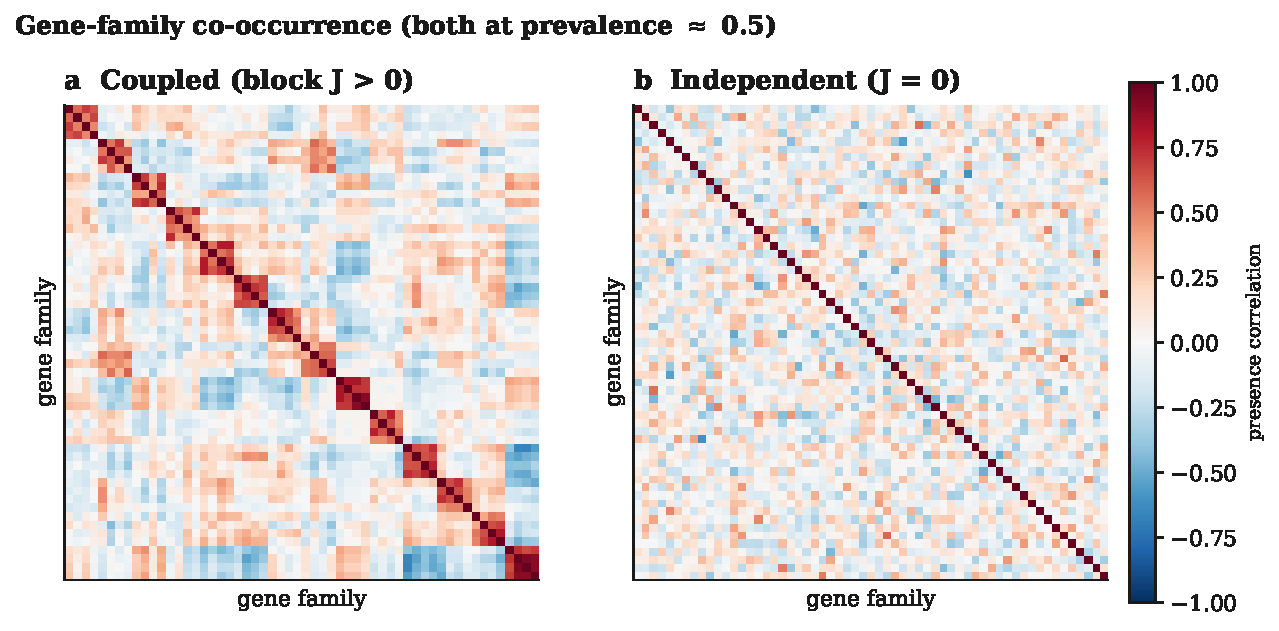
\includegraphics[width=\linewidth]{fig1_heatmaps.pdf}
\caption{Each square shows how often two gene families are present together across genomes (red\,=\,together, blue\,=\,apart), for the same number of genes at the same overall commonness. Coupling creates blocks of genes that travel together (a); without coupling there are none (b).}
\label{fig:heat}
\end{figure}

\textbf{ABC recovers the coupling strength.} Feeding simulated data to the method, the estimated
coupling tracks the true coupling across the whole range, with the truth inside every uncertainty
interval (Fig.~\ref{fig:rec}; typical error $\approx\,$\textbf{0.06} on a $0$--$1.5$ scale). So the
strength of coupling really is measurable from a presence/absence table alone.

\begin{figure}[h]\centering
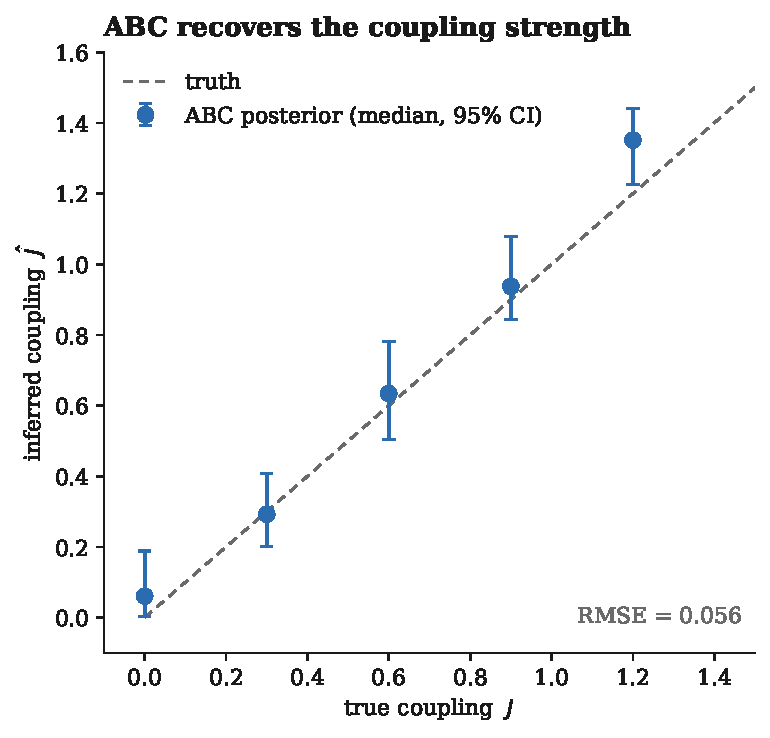
\includegraphics[width=0.56\linewidth]{fig2_recover_realistic.pdf}
\caption{Estimated vs.\ true coupling strength $J$ on simulated data (dot\,=\,best estimate, bar\,=\,95\% uncertainty). The dashed line is a perfect match.}
\label{fig:rec}
\end{figure}

\textbf{A subtlety worth understanding.} Coupling does two things at once: it makes coupled genes
\emph{more common}, and it makes them \emph{appear together}. So a method that only looks at
\emph{how common each gene is} can already sense coupling \emph{indirectly}, through commonness ---
which is why the estimates above work even without looking at co-occurrence. To find out whether
co-occurrence adds anything of its own, we ran a stricter test: we tuned the simulation so that genes
stay \emph{equally common no matter the coupling strength}, removing the ``commonness'' shortcut. Now
a method that only tracks gene commonness is helpless --- it cannot tell weak coupling from strong
(its error balloons to \textbf{0.37}). But a method that looks at \emph{which genes appear together}
still recovers the strength, roughly halving that error (Figs.~\ref{fig:cmp},~\ref{fig:pay}). The
lesson: gene commonness usually does the job, but co-occurrence is what saves you when it can't.

\begin{figure}[h]\centering
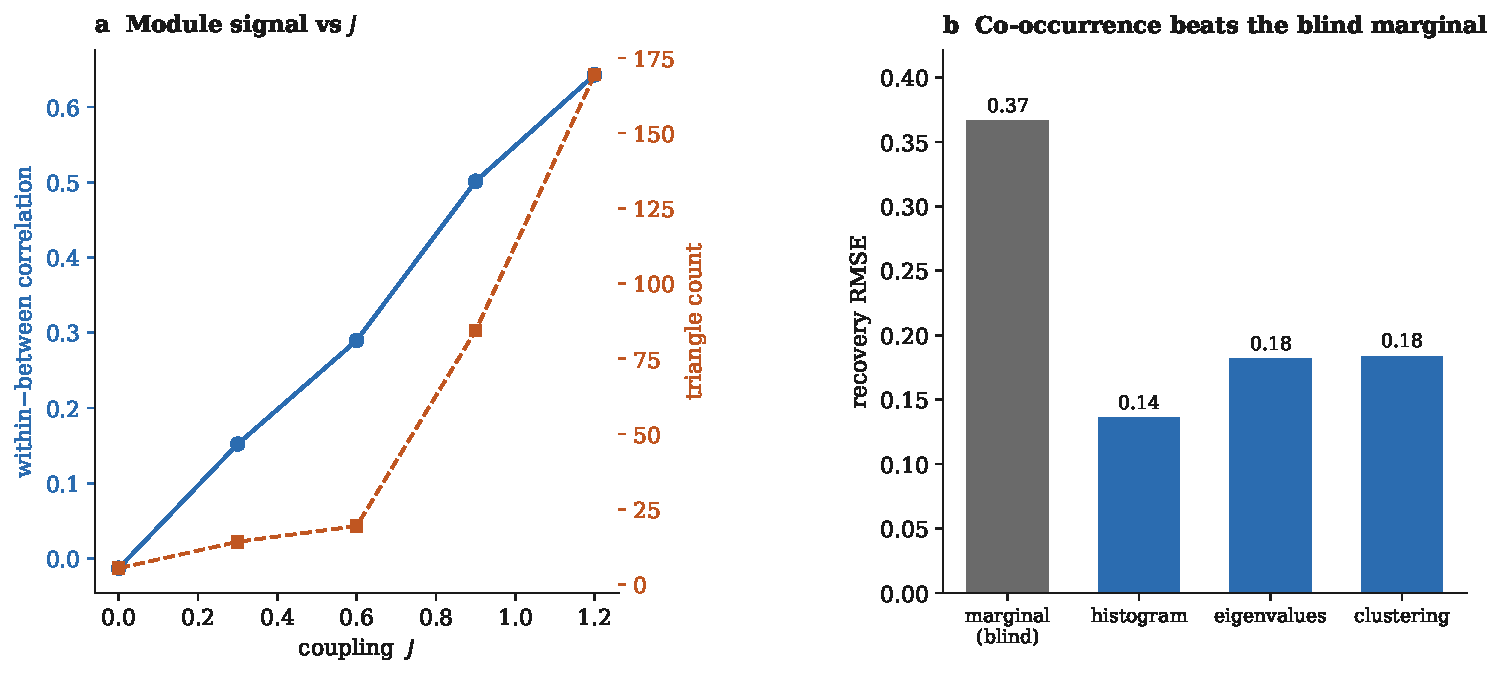
\includegraphics[width=\linewidth]{fig3_summary_comparison.pdf}
\caption{A \emph{simulation} experiment (60 species) with genes tuned to stay equally common regardless of coupling. (a) The co-occurrence signal still grows steadily with coupling strength. (b) Recovery error for four ways of reading the data, each averaged over several simulated datasets: reading only \emph{gene commonness} is blind here, while any method reading \emph{co-occurrence} roughly halves the error.}
\label{fig:cmp}
\end{figure}

\begin{figure}[h]\centering
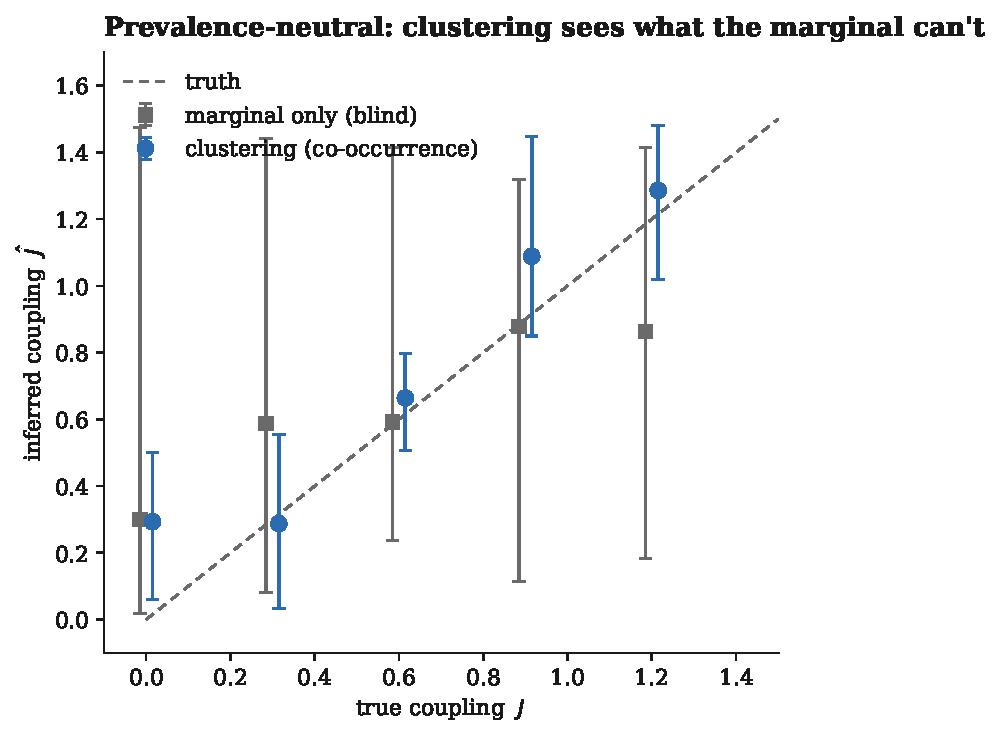
\includegraphics[width=0.56\linewidth]{fig4_recover_neutral.pdf}
\caption{Same stricter test, shown directly: reading only gene commonness (grey) is flat --- blind to the coupling; reading co-occurrence (blue) tracks the truth.}
\label{fig:pay}
\end{figure}

\section{Is coupling visible in real genomes?}

Now the real data: an eggNOG-annotated set of \textbf{43 bacterial genomes}. We group genes into
families (12{,}282 of them) and label each family by its broad \emph{function} (the COG functional
category --- translation, cell motility, energy metabolism, and so on). If coupling is real and
follows function, then \emph{genes of the same function should appear together more than genes of
different functions}. That is exactly what we test.

\textbf{Same-function genes travel together.} They do, and unmistakably. Comparing genes of the same
function against genes of different functions, same-function genes co-occur far more than one would
get by shuffling the function labels (Fig.~\ref{fig:emp}b; the shuffling keeps each gene's real
presence pattern, so it is not an artefact of the family tree). The effect is large and highly
significant ($p\approx\,$\textbf{0.002}).

\begin{figure}[h]\centering
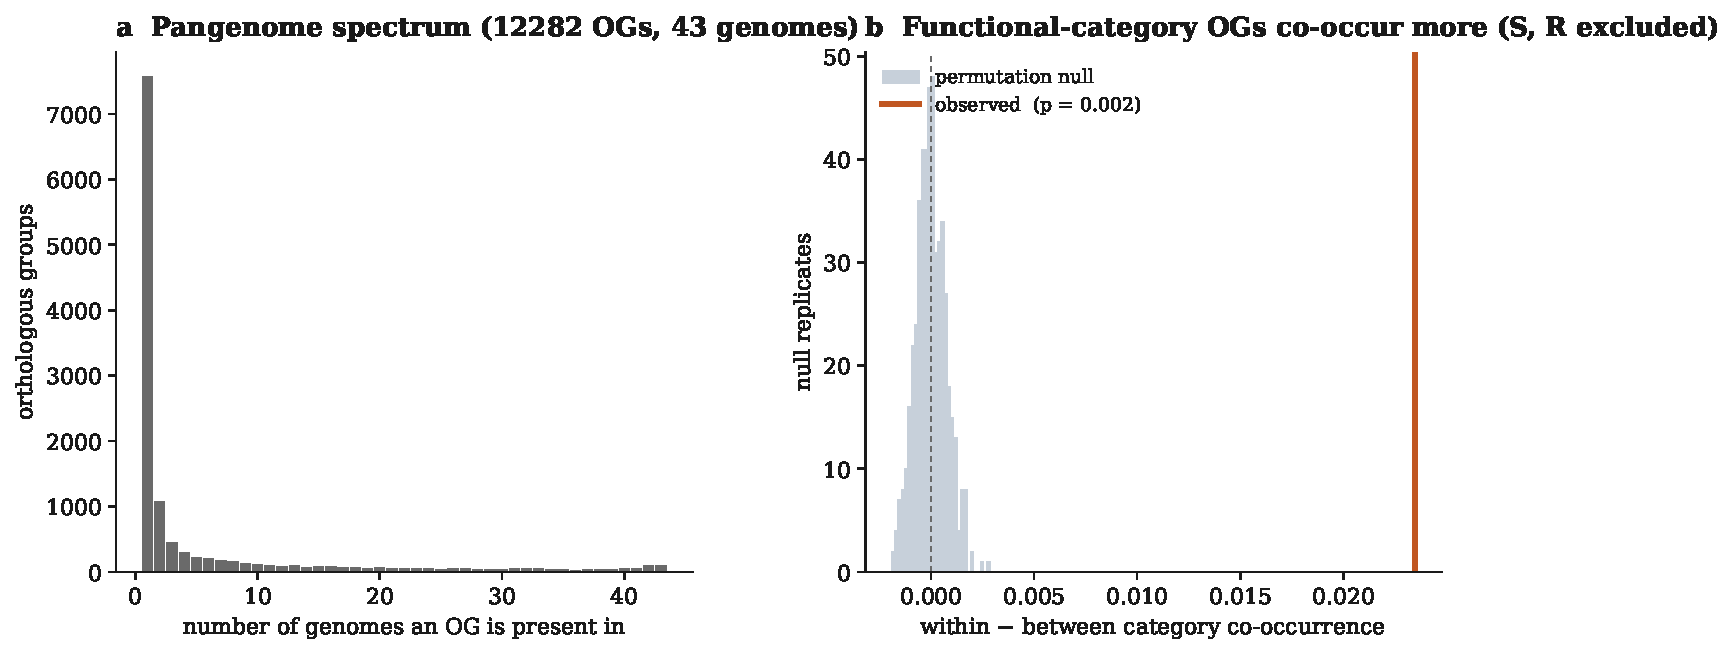
\includegraphics[width=\linewidth]{fig5_empirical.pdf}
\caption{Real eggNOG data (43 genomes). (a) Most gene families are found in only a few genomes; a small core is nearly universal. (b) Genes of the \emph{same} function appear together far more than if function were assigned at random.}
\label{fig:emp}
\end{figure}

\textbf{Which functions?} The signal is concentrated in exactly the functions biology would predict
(Fig.~\ref{fig:coh}). \emph{Cell motility} stands far above the rest --- the genes that build a
flagellum are a textbook example of a module that is inherited as a unit --- followed by nucleotide,
coenzyme, ion-transport, secretion and carbohydrate metabolism. Twelve of eighteen functions co-occur
significantly more than a random group of genes; the exceptions are functions like replication whose
genes are nearly universal and so cannot vary together. (We set aside the ``function unknown''
category from the start: it is not a coherent function and cannot be a module.)

\begin{figure}[h]\centering
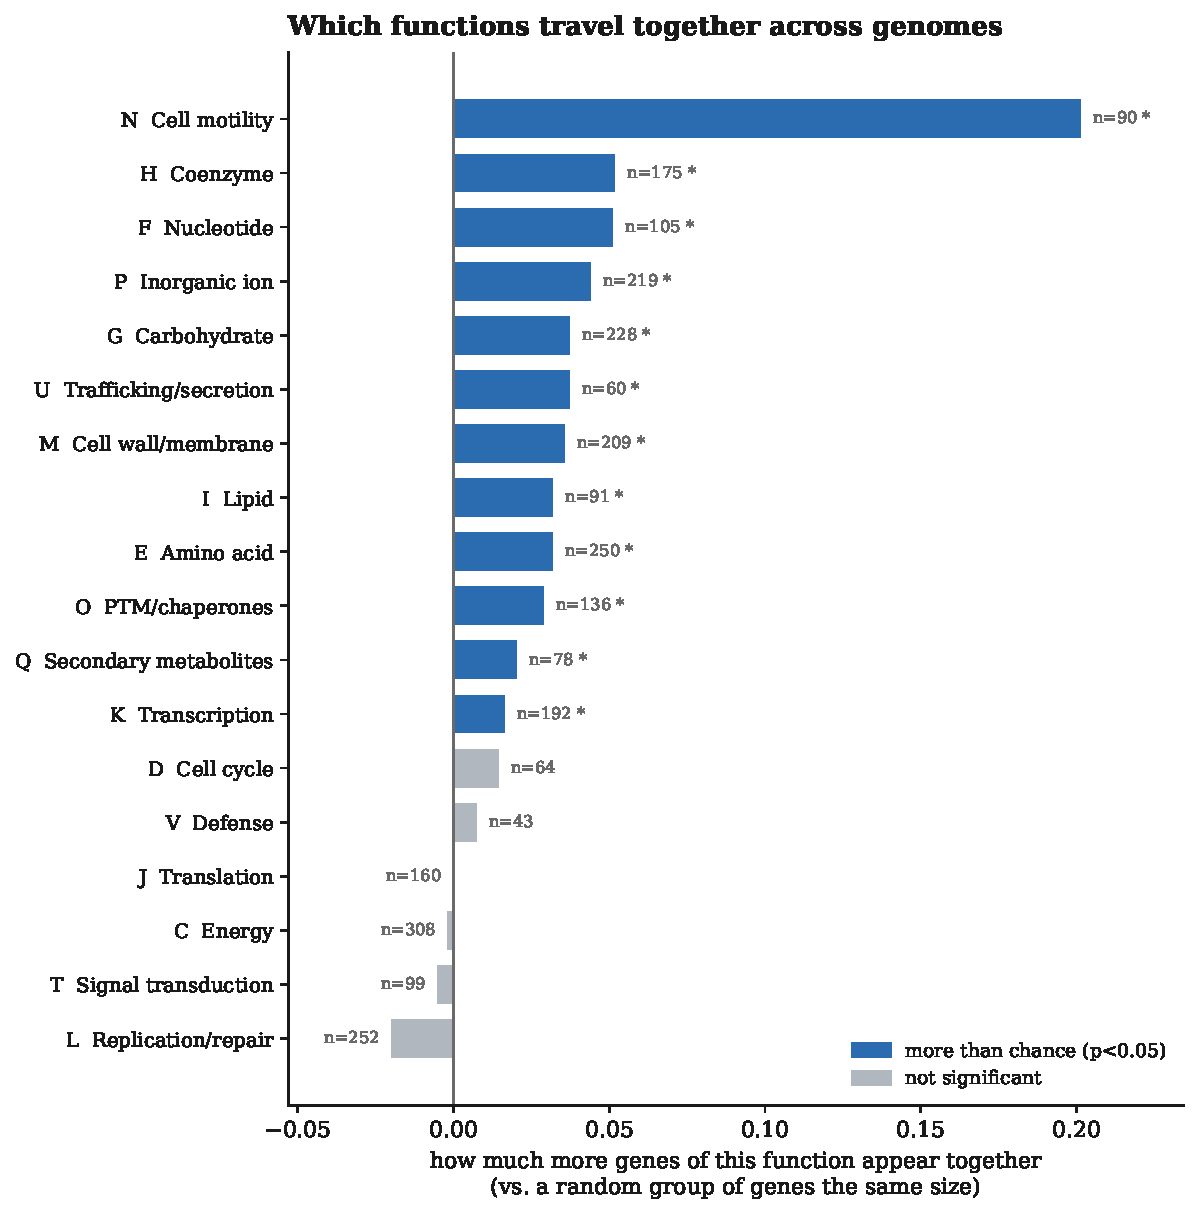
\includegraphics[width=0.82\linewidth]{fig6_cohesion.pdf}
\caption{How much more genes of each function appear together than a random group of the same size. Cell motility dominates; twelve of eighteen functions are significant (blue).}
\label{fig:coh}
\end{figure}

\section{What this means, and what is next}

\begin{itemize}\setlength\itemsep{0.2em}
\item \textbf{Coupling strength is measurable} from a presence/absence table (simulation error
$\approx\,0.06$), even though the model has no usable likelihood.
\item \textbf{Two signals, use both.} Coupling shows up in \emph{how common} genes are \emph{and} in
\emph{which genes appear together}. The first usually suffices; the second is essential when coupling
does not change how common genes are.
\item \textbf{Real genomes show functional coupling.} On 43 real bacterial genomes, same-function
genes appear together far more than chance ($p\approx0.002$), led overwhelmingly by cell motility.
\item \textbf{The next step: use function as the blueprint.} Rather than guessing which genes are
coupled, we can take genes of the same function as the coupled groups and fit the coupling
\emph{strength} for each function --- exactly the procedure this report validates. With the 43-genome
dataset now fully annotated, that fit is the immediate next milestone.
\end{itemize}

\vspace{0.4em}
{\small\color{muted}Reproducible: \texttt{analyses/coupling\_abc/run\_analysis.py} (simulation, Figs.~1--4) and \texttt{empirical\_analysis.py} (real data, Figs.~5--6); all results use fixed random seeds.}

\end{document}
